\documentclass[tikz,border=0pt]{standalone}
\usepackage{amsmath,amssymb}
\usepackage{newtxtext,newtxmath}
\usepackage{adjustbox}
\usetikzlibrary{arrows.meta,calc,decorations.pathreplacing}
\definecolor{deepblue}{HTML}{2F528F}
\definecolor{arrowblue}{HTML}{4472C4}
\definecolor{canvasbg}{HTML}{F3F6FA}
\definecolor{panelbg}{HTML}{FAFCFF}
\definecolor{boxbg}{HTML}{FFFFFF}

\begin{document}
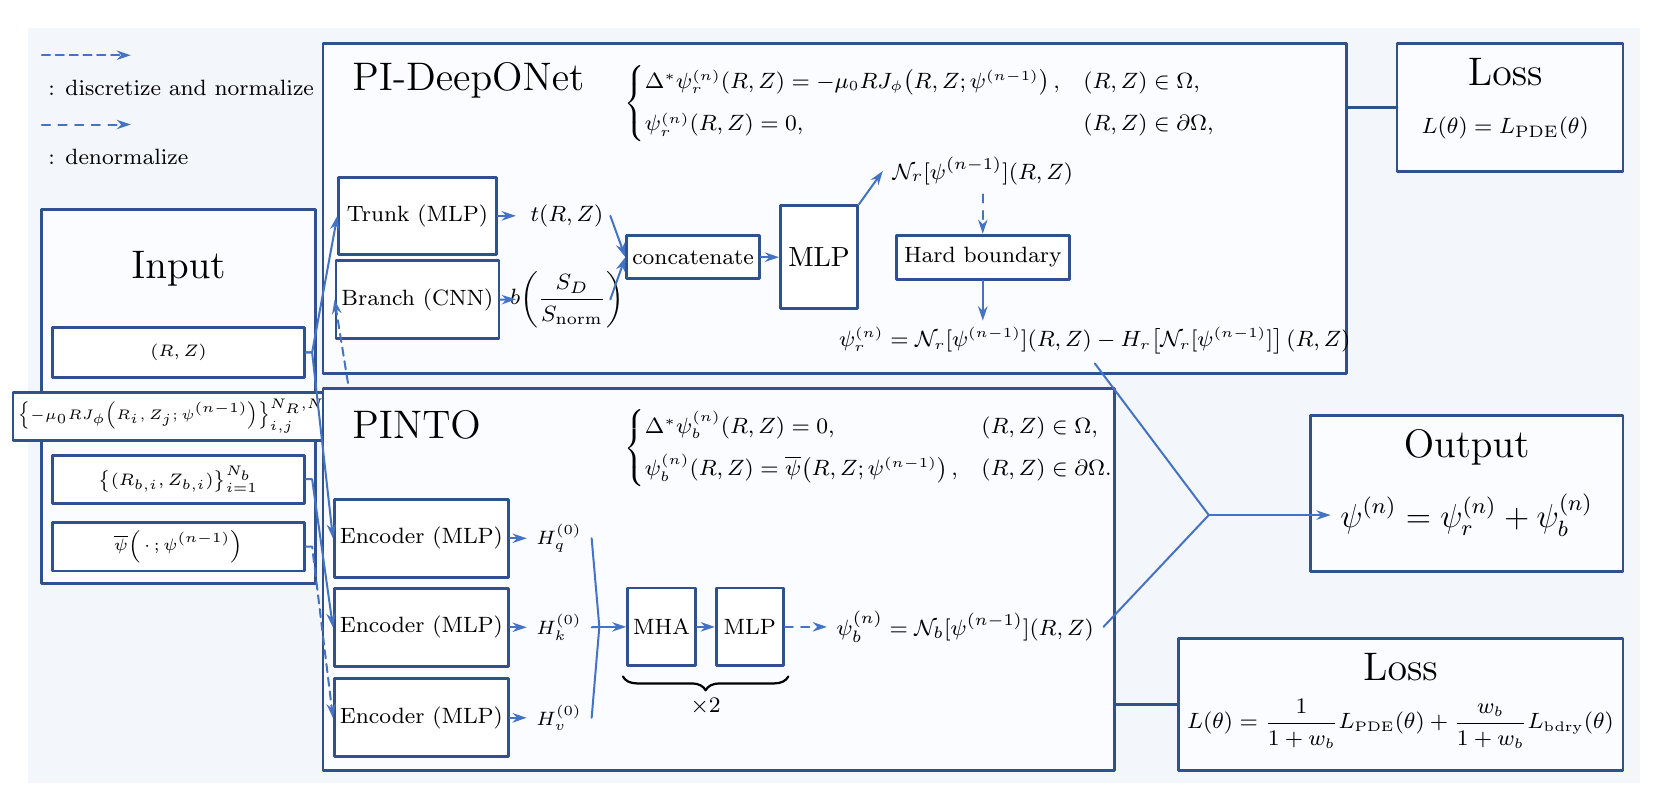
\begin{tikzpicture}[panel/.style={draw=deepblue, line width=1.05pt, fill=panelbg},
  drawline/.style={draw=deepblue, line width=1.00pt},
  box/.style={draw=deepblue, line width=1.00pt, fill=boxbg, align=center,
              inner sep=2pt, font=\fontsize{8.4}{10}\selectfont},
  flow/.style={draw=arrowblue, line width=.72pt,
               -{Stealth[length=1.8mm,width=1.2mm]}},
  prep/.style={flow, densely dashed},
  denorm/.style={flow, dashed},
  plainflow/.style={draw=arrowblue, line width=.72pt},
  title/.style={font=\fontsize{13.5}{15.5}\selectfont},
  eq/.style={font=\fontsize{8.5}{10.2}\selectfont},
  smallEq/.style={font=\fontsize{7.7}{9.3}\selectfont},
  x=1cm,y=1cm, line cap=round, line join=round]
  % Fixed canvas and subtle background
  \path[use as bounding box] (0,0) rectangle (20.48,9.59);
  \fill[canvasbg] (0,0) rectangle (20.48,9.59);

  % --------------------------------------------------------------------------
  % Legend
  % --------------------------------------------------------------------------
  \draw[prep]   (0.18,9.24) -- (1.31,9.24);
  \node[anchor=west,font=\fontsize{8.3}{10}\selectfont] at (0.14,8.83)
    {: discretize and normalize};
  \draw[denorm] (0.18,8.36) -- (1.31,8.36);
  \node[anchor=west,font=\fontsize{8.3}{10}\selectfont] at (0.14,7.95)
    {: denormalize};

  % --------------------------------------------------------------------------
  % Input panel
  % --------------------------------------------------------------------------
  \draw[panel] (0.18,2.53) rectangle (3.65,7.28);
  \node[title] at (1.915,6.53) {Input};

  \node[box,minimum width=3.2cm,minimum height=.63cm,
        font=\fontsize{6.5}{8.4}\selectfont] (inRZ) at (1.915,5.465)
    {$\displaystyle (R,Z)$};
  \node[box,minimum width=3.2cm,minimum height=.61cm,
        font=\fontsize{5.5}{8.4}\selectfont] (inSrc) at (1.915,4.655)
    {$\displaystyle
      \left\{-\mu_0 R J_\phi\!\left(R_i,Z_j;\psi^{(n-1)}\right)\right\}_{i,j}^{N_R,N_Z}$};
  \node[box,minimum width=3.2cm,minimum height=.61cm,
        font=\fontsize{6.5}{8.4}\selectfont] (inBnd) at (1.915,3.855)
    {$\displaystyle \left\{(R_{b,i},Z_{b,i})\right\}_{i=1}^{N_b}$};
  \node[box,minimum width=3.2cm,minimum height=.62cm,
        font=\fontsize{6.5}{8.4}\selectfont] (inPsi) at (1.915,3.000)
    {$\displaystyle \overline{\psi}\!\left(\,\cdot\,;\psi^{(n-1)}\right)$};

  % --------------------------------------------------------------------------
  % PI-DeepONet panel
  % --------------------------------------------------------------------------
  \draw[panel] (3.75,5.20) rectangle (16.75,9.39);
  \node[anchor=west,title] at (4,8.92) {PI-DeepONet};

  \node[anchor=north west,smallEq,align=left] (residualEq) at (7.46,9.24) {$\displaystyle
    \begin{cases}
      \Delta^{*}\psi_r^{(n)}(R,Z)
      =-\mu_0 R J_\phi\!\left(R,Z;\psi^{(n-1)}\right),
      & (R,Z)\in\Omega,\\[1.5mm]
      \psi_r^{(n)}(R,Z)=0,
      & (R,Z)\in\partial\Omega,
    \end{cases}$};

  \node[box,minimum width=2cm,minimum height=.98cm] (trunk) at (4.95,7.2)
    {Trunk (MLP)};
  \node[box,minimum width=2cm,minimum height=.99cm] (branch) at (4.95,6.135)
    {Branch (CNN)};

  \node[eq] at (6.85,7.205) {$\displaystyle t(R,Z)$};
  \node[eq] at (6.85,6.140)
    {$\displaystyle b\!\left(\frac{S_D}{S_{\mathrm{norm}}}\right)$};
  \node[box,minimum width=1.3cm,minimum height=.55cm] (concat) at (8.45,6.675)
  {concatenate};
%   \draw[panel,fill=boxbg] (6.7,5.61) rectangle (8.0,7.74);
%   \draw[deepblue,line width=1.00pt] (6.7,6.67) -- (8.0,6.67);

  \node[box,minimum width=.98cm,minimum height=1.31cm,
        font=\fontsize{9.6}{11.5}\selectfont] (topmlp) at (10.05,6.675) {MLP};
  \node[eq] (nr) at (12.13,7.770)
    {$\displaystyle \mathcal{N}_r[\psi^{(n-1)}](R,Z)$};

  \node[box,minimum width=2.2cm,minimum height=.56cm,
        font=\fontsize{8.5}{10.2}\selectfont] (hardbdry) at (12.13,6.675)
    {Hard boundary};

  \node[anchor=west,font=\fontsize{7.7}{9.2}\selectfont] (residual) at (10.18,5.62) {$\displaystyle
    \psi_r^{(n)}
    =\mathcal{N}_r[\psi^{(n-1)}](R,Z)
     -H_r\!\left[\mathcal{N}_r[\psi^{(n-1)}]\right](R,Z)$};

  % PI-DeepONet flow
  \draw[flow] (trunk.east) -- (6.2,7.20);
  \draw[flow] (branch.east) -- (6.2,6.14);
  \draw[flow] (7.4,7.20) -- (concat.west);
  \draw[flow] (7.4,6.14) -- (concat.west);
  \draw[flow] (concat.east) -- (topmlp.west);
  \draw[flow] (topmlp.north east) -- (nr.west);
  \draw[denorm] (nr.south) -- (hardbdry.north);
  \draw[flow] (hardbdry.south) -- (12.13,5.87);

  % Inputs to PI-DeepONet
  \draw[flow] (inRZ.east) -- ++(.08,0) -- (trunk.west);
  \draw[prep] (inSrc.east) -- ++(.10,0) -- (branch.west);

  % --------------------------------------------------------------------------
  % PINTO panel
  % --------------------------------------------------------------------------
  \draw[panel] (3.75,0.16) rectangle (13.80,5.01);
  \node[anchor=west,title] at (4,4.54) {PINTO};

  \node[anchor=north west,smallEq,align=left] (boundaryEq) at (7.46,4.86) {$\displaystyle
    \begin{cases}
      \Delta^{*}\psi_b^{(n)}(R,Z)=0,
      & (R,Z)\in\Omega,\\[1.5mm]
      \psi_b^{(n)}(R,Z)
      =\overline{\psi}\!\left(R,Z;\psi^{(n-1)}\right),
      & (R,Z)\in\partial\Omega.
    \end{cases}$};

  \node[box,minimum width=2.1cm,minimum height=.99cm] (encq) at (5,3.105)
    {Encoder (MLP)};
  \node[box,minimum width=2.1cm,minimum height=.99cm] (enck) at (5,1.975)
    {Encoder (MLP)};
  \node[box,minimum width=2.1cm,minimum height=.99cm] (encv) at (5,.825)
    {Encoder (MLP)};

  \node[eq,minimum width=.70cm,minimum height=.99cm,
        font=\fontsize{7.5}{10.2}\selectfont] (hq) at (6.75,3.105)
    {$\displaystyle H_q^{(0)}$};
  \node[eq,minimum width=.70cm,minimum height=.99cm,
        font=\fontsize{7.5}{10.2}\selectfont] (hk) at (6.75,1.975)
    {$\displaystyle H_k^{(0)}$};
  \node[eq,minimum width=.70cm,minimum height=.99cm,
        font=\fontsize{7.5}{10.2}\selectfont] (hv) at (6.75,.825)
    {$\displaystyle H_v^{(0)}$};

  \node[box,minimum width=.85cm,minimum height=.99cm,
        font=\fontsize{8.4}{11.5}\selectfont] (mha) at (8.05,1.98) {MHA};
  \node[box,minimum width=.85cm,minimum height=.99cm,
        font=\fontsize{8.4}{11.5}\selectfont] (botmlp) at (9.17,1.98) {MLP};

  \node[anchor=west,font=\fontsize{7.9}{9.5}\selectfont] (boundary) at (10.15,1.98) {$\displaystyle
    \psi_b^{(n)}=\mathcal{N}_b[\psi^{(n-1)}](R,Z)$};

  % PINTO flow
  \draw[flow] (encq.east) -- (hq.west);
  \draw[flow] (enck.east) -- (hk.west);
  \draw[flow] (encv.east) -- (hv.west);

  \coordinate (attnJoin) at (7.26,1.98);
  \draw[plainflow] (hq.east) -- (attnJoin);
  \draw[plainflow] (hk.east) -- (attnJoin);
  \draw[plainflow] (hv.east) -- (attnJoin);
  \draw[flow] (attnJoin) -- (mha.west);
  \draw[flow] (mha.east) -- (botmlp.west);
  \draw[denorm] (botmlp.east) -- (boundary.west);

  \draw[decorate,decoration={brace,mirror,amplitude=5pt},line width=.8pt]
    (7.56,1.35) -- (9.66,1.35)
    node[midway,below=4pt,font=\fontsize{8.5}{9.7}\selectfont] {$\times 2$};

  % Inputs to PINTO: query, key and value streams
  \draw[flow] (inRZ.east) -- ++(.08,0) -- (encq.west);
  \draw[flow] (inBnd.east) -- ++(.08,0) -- (enck.west);
  \draw[prep] (inPsi.east) -- ++(.08,0) -- (encv.west);

  % --------------------------------------------------------------------------
  % Right-hand output and losses
  % --------------------------------------------------------------------------
  \draw[panel] (17.39,7.76) rectangle (20.26,9.39);
  \node[title] at (18.765,9.03) {Loss};
  \node[eq] (pideeopneteq) at (18.765,8.31)
    {$\displaystyle L(\theta)=L_{\mathrm{PDE}}(\theta)$};

  \draw[panel] (16.29,2.68) rectangle (20.26,4.66);
  \node[title] at (18.275,4.26) {Output};
  \node[font=\fontsize{11.5}{13.8}\selectfont] (output) at (18.275,3.4)
    {$\displaystyle \psi^{(n)}=\psi_r^{(n)}+\psi_b^{(n)}$};

  \draw[panel] (14.61,.16) rectangle (20.26,1.83);
  \node[title] at (17.435,1.47) {Loss};
  \node[smallEq] (pintoeq) at (17.435,0.75) {$\displaystyle
    L(\theta)=\frac{1}{1+w_b}L_{\mathrm{PDE}}(\theta)
    +\frac{w_b}{1+w_b}L_{\mathrm{bdry}}(\theta)$};
  \coordinate (outputjoin) at (15,3.4);
  \draw[plainflow] (residual.south) -- (outputjoin);
%   \draw[] (residualEq.east) -- (pideeopneteq.west);
  \draw[drawline] (16.75,8.575) -- (17.39,8.575);
  \draw[plainflow] (boundary.east) -- (outputjoin);
  \draw[flow] (outputjoin) -- (output.west);
  \draw[drawline] (13.80,0.995) -- (14.61,0.995);

\end{tikzpicture}
\end{document}